% siminos/atlas/symm.tex  pdflatex atlas
% $Author$ $Date$

\section{Dancers and drifters}
% and symmetries}
% Dynamics and symmetry
\label{s:symm}

%% A27*-pipeSymms.* - read dasbuch/book/FigSrc/inkscape/00ReadMe.txt
 \begin{figure}
 \begin{center}
  \setlength{\unitlength}{0.20\textwidth}
  %% \unitlength = units used in the Picture Environment
(a)
  \begin{picture}(1,0.52454249)%
    \put(0,0){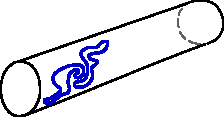
\includegraphics[width=\unitlength]{A27a-pipeSymms}}%
    \put(0.61583231,0.13683004){\color[rgb]{0,0,0}\makebox(0,0)[lb]{\smash{$z$}}}%
    \put(0.00611823,0.27217453){\color[rgb]{0,0,0}\makebox(0,0)[lb]{\smash{$\theta$}}}%
  \end{picture}%
(b)
  \begin{picture}(1,0.52454249)%
    \put(0,0){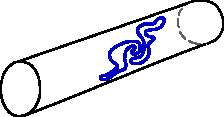
\includegraphics[width=\unitlength]{A27b-pipeSymms}}%
    \put(0.61583231,0.13683004){\color[rgb]{0,0,0}\makebox(0,0)[lb]{\smash{$z$}}}%
    \put(0.00611823,0.27217453){\color[rgb]{0,0,0}\makebox(0,0)[lb]{\smash{$\theta$}}}%
  \end{picture}%
\\
(c)
  \begin{picture}(1,0.52454249)%
    \put(0,0){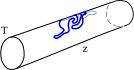
\includegraphics[width=\unitlength]{A27c-pipeSymms}}%
    \put(0.61583231,0.13683004){\color[rgb]{0,0,0}\makebox(0,0)[lb]{\smash{$z$}}}%
    \put(0.00611823,0.27217453){\color[rgb]{0,0,0}\makebox(0,0)[lb]{\smash{$\theta$}}}%
  \end{picture}%
(d)
  \begin{picture}(1,0.52454249)%
    \put(0,0){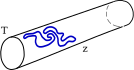
\includegraphics[width=\unitlength]{A27d-pipeSymms}}%
    \put(0.61583231,0.13683004){\color[rgb]{0,0,0}\makebox(0,0)[lb]{\smash{$z$}}}%
    \put(0.00611823,0.27217453){\color[rgb]{0,0,0}\makebox(0,0)[lb]{\smash{$\theta$}}}%
  \end{picture}%
 \end{center}
 \caption[$\On{2}_\theta \times \SOn{2}_z$ symmetry of flow in a stream-wise
          periodic pipe]{
A fluid state in a pipe translated or rotated is
also a solution. In particular, a \rpo\ $\pS_p$ is
(a) a \emph{time dependent} state of the fluid that after a period $\period{p}$ reemerges
(b) translated by downstream shift $\shift_p$
(such solutions are stream-wise periodic pipe $\SOn{2}_z$ equivariant),
(c) translated by downstream shift $\shift_p$ and rotated azimuthally by $\gSpace_p$
(i.e., $\SOn{2}_{\phi} \times \SOn{2}_z$ equivariant) or,
(d) reflected and rotated azimuthally by $\gSpace$ (i.e., $\On{2}_{\phi}$ equivariant).
Consider this in contrast to a \reqv, a constant shape that travels
downstream with constant {\phaseVel} $\velRel$. (from \wwwcb{})
 }\label{fig:A27-pipeSymms}
 \end{figure}
%% A27*-pipeSymms.* %%%%%%%%%%%%%%%%%%%%%%%%%%%%%%%%%%%%%%%%%%%%%%%%%%%%%%%

What is a symmetry? A visualization of the fluid dynamics of a pipe flow,
\reffig{fig:A27-pipeSymms}, affords an intuitive illustration. Solutions
of pipe flow remain physically the same under azimuthal rotations and
stream-wise translations (which become \SOn{2} rotations in numerical
stream-wise periodic pipes) but correspond to different points in
\statesp\ and may look very different in its visualizations.

Each \SOn{2} group orbit is topologically a circle, but it traces out a
complicated \statesp\ curve composed of many Fourier modes nonlinearly
coupled and thus of comparable magnitudes. Together
the two \SOn{2} sweep out contorted and hard to visualize $T^2$ tori (see
\refref{ACHKW11}), but we shall illustrate here the key ideas by a much
simpler example, the $\SOn{2}$-equivariant Gibbon and
McGuinness\rf{GibMcCLE82,FowlerCLE82} \cLe\ of geophysics and laser
physics,
\bea
	\dot{x}_1 &=& -\sigma x_1 + \sigma y_1
        \,,\qquad
	\dot{x}_2 \,=\, -\sigma x_2 + \sigma y_2
        \continue
	\dot{y}_1 &=& (\RerCLor-z) x_1 - \ImrCLor x_2 -y_1-e y_2 \continue
	\dot{y}_2 &=& \ImrCLor x_1 + (\RerCLor-z) x_2 + e y_1- y_2\continue
	\dot{z} \; &=& -b z + x_1 y_1 + x_2 y_2
    \,.
\label{eq:CLeR}
\eea
Here the parameters are set to Siminos's values $\RerCLor=28,\,
\ImrCLor=0,\, b=8/3,\, \sigma=10,\, e= 1/10$. (For the background and an
in-depth investigation of the model  see \refrefs{SiminosThesis,SiCvi10}.)

\begin{figure}
  	\begin{center}
  	\setlength{\unitlength}{0.20\textwidth}
  (a)
  	\begin{picture}(1,1.07802818)%
    	\put(0,0){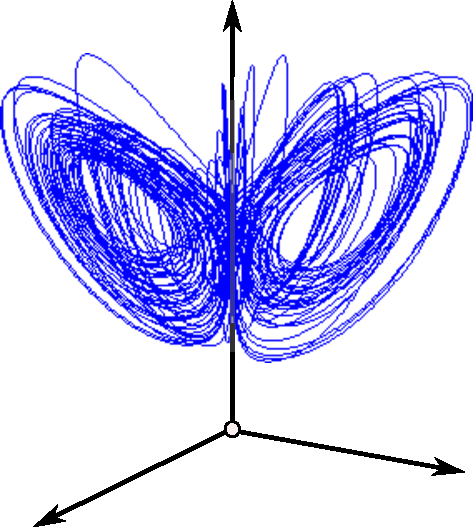
\includegraphics[width=\unitlength]{CLEattractor}}%
    	\put(0.55152995,1.0139628){\color[rgb]{0,0,0}\makebox(0,0)[lb]{\smash{$z$}}}%
    	\put(0.05573445,0.0739776){\color[rgb]{0,0,0}\makebox(0,0)[lb]{\smash{$x_1$}}}%
    	\put(0.90013492,0.16491708){\color[rgb]{0,0,0}\makebox(0,0)[lb]{\smash{$x_2$}}}%
  	\end{picture}%	
  (b)
  	\begin{picture}(1,1.06440474)%
    	\put(0,0){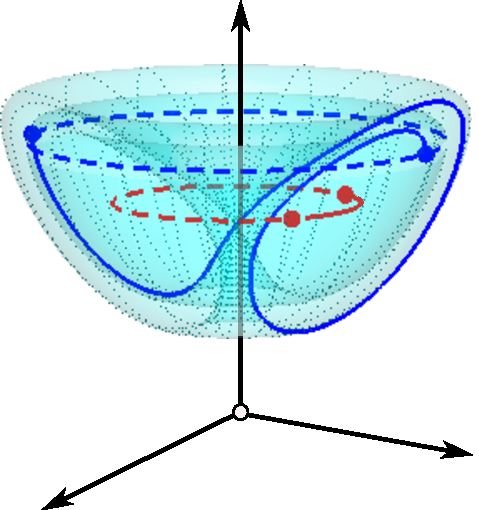
\includegraphics[width=\unitlength]{CLEWurst01}}%
   		\put(0.55961552,1.00214901){\color[rgb]{0,0,0}\makebox(0,0)[lb]{\smash{$z$}}}%
   		\put(0.07008555,0.07304272){\color[rgb]{0,0,0}\makebox(0,0)[lb]{\smash{$x_1$}}}%
    	\put(0.90381504,0.16283301){\color[rgb]{0,0,0}\makebox(0,0)[lb]{\smash{$x_2$}}}%
  	\end{picture}	
    \end{center}
  \caption
  [\CLf: $\cycle{01}$ {\rpo} group orbit]{
  (a)
  The strange attractor of \cLf.
  (b)
  The initial \reqv\ $\REQV{}{1}$ point is shown by the red dot, and its
  group orbit / trajectory by the dashed red line. One period of the
  $\cycle{01}$ {\rpo} is shown by the solid blue line. The group orbit of
  its (arbitrary) starting point is shown by the dashed blue line: after
  one period the trajectory has returned to the group orbit but with a
  different phase. The wurst, \ie, the group orbit of the $\cycle{01}$
  trajectory (dark blue) is shown by the cyan surface. Trajectory of the
  further 15 repeats of $\cycle{01}$ (faint dotted lines) traces out this
  torus; in that time the slowly drifting \reqv\ $\REQV{}{1}$ has
  advanced to the next red dot (red line).
  }
\label{fig:CLf01group}
\end{figure}

The strange attractor of the \cLf\ is shown in
\reffig{fig:CLf01group}\,(a). It is a mess. Why? The problem of dynamics
in presence of symmetry can perhaps be understood this way: dissipative
flows settle into solutions with low friction. Since drifting along the
non-shape-changing symmetry directions is energetically cheap, rather
than do work, solutions tend to drift along. Thus, the physically
important shape-changing dynamics are smeared out.
%DB 4/13/2012: I think this is the general idea, but not sure how much of a claim this is
    \KC{2012-04-13}{I do not understand the paragraph. Predrag: did
                    Daniel's edit help?}

A continuous symmetry leads to drifting invariant solutions. A {\em
\reqv} (traveling wave, rotational wave, ...) is a trajectory whose
velocity field lies within the group tangent space, such that
\(
\vel(\ssp) = c \cdot \groupTan(\ssp)
\) %\label{phaseVel}
with a constant {\phaseVel} $c$, and whose time evolution is thus
confined to the group orbit; think of an unchanging body carried by a
stream.

A {\em \rpo} $\pS_p$ is a trajectory which exactly recurs
\beq
\ssp(\zeit) = \LieEl_p \, \ssp(\zeit + \period{p} )
    \,,\qquad
\ssp(\zeit) \in \pS_p
\ee{RPOrelper1}
after a fixed {relative period} $\period{p}$, but shifted by a fixed
group action ${\LieEl}$ that maps the endpoint $\ssp (\period{p}) $ back
into the initial point cycle point $\ssp (0) $; think of a dancer moving
across the stage through a set of motions and then striking the initial
pose\rf{ShWi06}, or study the pipe flow sketches \reffig{fig:A27-pipeSymms}.

As the $\SOn{2}$ transformations act on the \cLf\ only through the
simplest, $m=1$ Fourier mode, here all group orbits are circles, and appear
elliptical in most $d=5 \to 3$~dimensions projections. Nevertheless, even
the wurst traced out by the very simplest, short \rpo\ $\cycle{01}$ shown
in \reffig{fig:CLf01group}\,(b) is not so easy to get one's head around:
you are looking at a 3\dmn\ projection of a \emph{torus} embedded in 5
dimensions.

%%%%%%%%%%%%%%%%%%%%%%%%%%%%%%%%%%%%%%%%%%%%%%%%%
% 2011-09-09, 2012-03-30 Predrag: add BeThMovFr to
%            continuous.tex overheads, and ChaosBook
% replace A27movFrame*.* everywhere
\begin{figure}
 \begin{center}
  \setlength{\unitlength}{0.20\textwidth}
  %% \unitlength = units used in the Picture Environment
(a)~~
  \begin{picture}(1,0.98655417)%
    \put(0,0){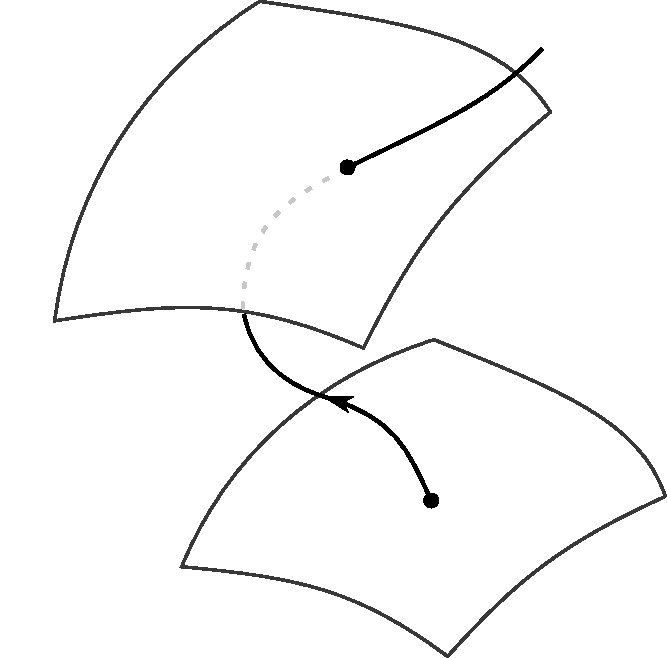
\includegraphics[width=\unitlength]{BeThTrajTeX}}%
    \put(0.35976094,0.91875614){\color[rgb]{0,0,0}\rotatebox{-31.32889204}{\makebox(0,0)[lb]{\smash{$\pS_{\ssp(\zeit)}$}}}}%
        \put(0.60333631,0.42274457){\color[rgb]{0,0,0}\rotatebox{-40.8073288}{\makebox(0,0)[lb]{\smash{$\pS_{\ssp(0)}$}}}}%
    \put(0.66001383,0.16959019){\color[rgb]{0,0,0}\rotatebox{0.0313674}{\makebox(0,0)[lb]{\smash{$\ssp(0)$}}}}%
    \put(0.5058276,0.64524238){\color[rgb]{0,0,0}\rotatebox{0.0313674}{\makebox(0,0)[lb]{\smash{$\ssp(\zeit)$}}}}%
    \put(0.13110825,0.05766516){\color[rgb]{0,0,0}\rotatebox{0.11031334}{\makebox(0,0)[lb]{\smash{$\pS$}}}}%
  \end{picture}%
~~(b)
  \begin{picture}(1,0.98655417)%
    \put(0,0){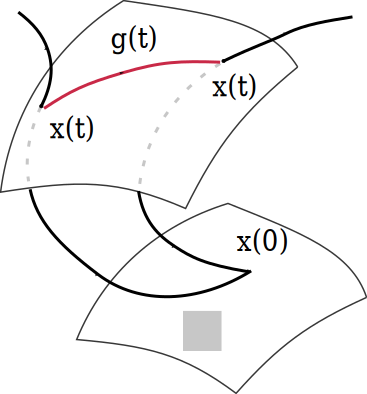
\includegraphics[width=\unitlength]{BeThMovFr}}%
    \put(0.20559239,0.64023845){\color[rgb]{0,0,0}\rotatebox{0.0313674}{\makebox(0,0)[lb]{\smash{$\ssp(\zeit)$}}}}%
    \put(0.67382401,0.35781161){\color[rgb]{0,0,0}\rotatebox{0.0313674}{\makebox(0,0)[lb]{\smash{$\ssp(0)$}}}}%
    \put(0.61221026,0.74589514){\color[rgb]{0,0,0}\rotatebox{0.0313674}{\makebox(0,0)[lb]{\smash{$\sspRed(\zeit)$}}}}%
    \put(0.35760559,0.8662057){\color[rgb]{0,0,0}\rotatebox{0.0313674}{\makebox(0,0)[lb]{\smash{$\LieEl(\zeit)$}}}}%
  \end{picture}%
 \end{center}
  \caption{\label{fig:BeThMovFr}
(a)
The group orbit $\pS_{\ssp(0)}$ of \statesp\ point $\ssp(0)$, and the
group orbit $\pS_{\ssp(\zeit)}$ reached by the trajectory $\ssp(\zeit)$ a time $\zeit$
later.
(b)
The two physically equivalent flows
$\ssp(\zeit)=\LieEl(\zeit)\,\sspRed(\zeit)$ are related by, in general,
an arbitrary, time dependent {\em moving frame} transformation
$\LieEl(\zeit)$.
(from \wwwcb{}).
  }
\end{figure}
%%%%%%%%%%%%%%%%%%%%%%%%%%%%%%%%%%%%%%%%%%%%%%%%%%

To summarize: continuous symmetries of dynamics stratify the \statesp\
into an onion, each layer a group orbit (\reffig{fig:BeThMovFr}). We are
free to replace a given flow $\ssp(\zeit)$ by another, physically
equivalent flow $\ssp(\zeit)=\LieEl(\zeit)\,\sspRed(\zeit)$ by any, in
general, time dependent {\em moving frame} transformation
$\LieEl(\zeit)$. For example, to film our dancer we can mount the camera
on a cart moving alongside her. So, in presence of continuous symmetries,
there are two kinds of change in time: a dancer, continuously changing
shapes, or a drifter, merely shuffling along the easy, shape non-changing
directions. We will presently banish the drifters, and just enjoy the
dance.
